% Design-grid figure (N vs design tokens-per-parameter), TikZ port of the paper's
% appendix TPP-grid schematic (labels grid:ncgrid / grid:tpp in the companion paper),
% re-keyed to this repo's grid. Hand-authored from the documented design spec in
% README.md / CLAUDE.md, exactly as the paper's grid was hand-drawn (no plotting script).
%
% Grid (matches data_final_metrics.csv: 29 envelope cells, 5 model sizes):
%   rows (bottom to top): N_nonembed = 57K, 397K, 10.6M, 85M, 354M
%   cols (left to right): design-TPP (D/N_total) = 20, 29, 43, 63, 93, 136, 200
%   Train  (blue): four lower rows, N <= 85M, 24 cells
%   Holdout (red): top row, 354M frontier, 5 cells
%   Unused (white): configs run at only 6 of 7 targets per size (largest at 5)
%
% Build: ./build_design_grid.sh  (writes ../design_grid.png)
\documentclass[border=8pt]{standalone}
\usepackage{tikz}
\begin{document}
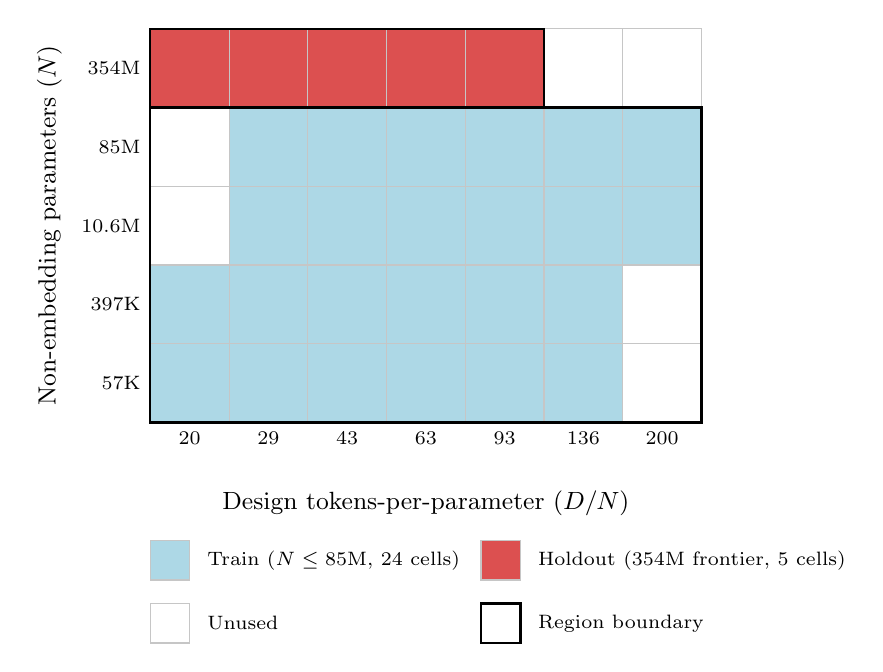
\begin{tikzpicture}[font=\sffamily]
  \definecolor{trainblue}{RGB}{173,216,230}
  \definecolor{holdoutred}{RGB}{220,80,80}

  % cell fills
  \foreach \x in {0,1,2,3,4,5}{ \fill[trainblue]  (\x,0) rectangle ++(1,1); } % 57K:  20 to 136
  \foreach \x in {0,1,2,3,4,5}{ \fill[trainblue]  (\x,1) rectangle ++(1,1); } % 397K: 20 to 136
  \foreach \x in {1,2,3,4,5,6}{ \fill[trainblue]  (\x,2) rectangle ++(1,1); } % 10.6M:29 to 200
  \foreach \x in {1,2,3,4,5,6}{ \fill[trainblue]  (\x,3) rectangle ++(1,1); } % 85M:  29 to 200
  \foreach \x in {0,1,2,3,4}  { \fill[holdoutred] (\x,4) rectangle ++(1,1); } % 354M: 20 to 93

  % lattice outlines (all 35 cells)
  \foreach \y in {0,...,4}{ \foreach \x in {0,...,6}{
    \draw[gray!45, thin] (\x,\y) rectangle ++(1,1); }}

  % region borders
  \draw[black, thick] (0,0) rectangle (7,4);  % training region (four lower rows)
  \draw[black, thick] (0,4) rectangle (5,5);  % holdout block (354M frontier)

  % x tick labels (design-TPP)
  \foreach \lab [count=\x from 0] in {20,29,43,63,93,136,200}{
    \node[below, font=\scriptsize] at (\x+0.5, 0) {\lab};
  }
  % y tick labels (non-embedding N)
  \foreach \lab [count=\y from 0] in {{57K},{397K},{10.6M},{85M},{354M}}{
    \node[left, font=\scriptsize] at (0, \y+0.5) {\lab};
  }

  % axis titles
  \node[below=0.75cm, font=\small] at (3.5, 0)
    {Design tokens-per-parameter ($D/N$)};
  \node[left=1.0cm, rotate=90, anchor=south, font=\small] at (0, 2.5)
    {Non-embedding parameters ($N$)};

  % legend
  \fill[trainblue] (0,-2.0) rectangle ++(0.5,0.5);
  \draw[gray!45, thin] (0,-2.0) rectangle ++(0.5,0.5);
  \node[right, font=\scriptsize] at (0.6,-1.75) {Train ($N\le 85$M, 24 cells)};

  \fill[holdoutred] (4.2,-2.0) rectangle ++(0.5,0.5);
  \draw[gray!45, thin] (4.2,-2.0) rectangle ++(0.5,0.5);
  \node[right, font=\scriptsize] at (4.8,-1.75) {Holdout (354M frontier, 5 cells)};

  \fill[white] (0,-2.8) rectangle ++(0.5,0.5);
  \draw[gray!45, thin] (0,-2.8) rectangle ++(0.5,0.5);
  \node[right, font=\scriptsize] at (0.6,-2.55) {Unused};

  \draw[black, thick] (4.2,-2.8) rectangle ++(0.5,0.5);
  \node[right, font=\scriptsize] at (4.8,-2.55) {Region boundary};
\end{tikzpicture}
\end{document}
